\section{Calibration of existing transformation models 校准现有的转换模型}

\begin{paracol}{2}
        
    In the database, there are data points where two or more clay parameters are simultaneously known. For instance, a disturbed clay sample is extracted to determine PI, and an undisturbed clay sample is extracted at a nearby borehole at the same depth to determine $s_u$. In this case, PI and $s_u$ are simultaneously known. These data points can be compared with transformation models proposed in literature as a rough check for consistency. Twentyfour transformation models shown in \autoref{table:5} are considered. Most of these models were developed based on certain clay databases, but these databases may not be global in the sense that the data are limited to certain clay types or certain geographic locations. In other words, they are typically site-specific models. It is recommended that the basic statistics of the database supporting the development of transformation models should be explicitly reported in the form of \autoref{table:3} and (or) \autoref{table:4}. The characteristics of the databases underlying numerous existing transformation models are not known and this complicates comparisons with other databases such as the one presented in this study. These characteristics are of interest, because engineers can make a more informed decision on the applicability of a particular transformation model to his or her design scenario at hand.
    
    \switchcolumn
        
    在数据库中,存在同时知道两个或多个黏土参数的数据点。例如,提取扰动的黏土样品以确定PI,并在附近井眼的相同深度提取未扰动的黏土样品以确定$s_u$。在这种情况下,PI和$s_u$同时为已知。这些数据点可以与文献中提出的转换模型进行比较,作为对一致性的粗略检查。考虑了\cntableref{table:5}中所示的二十四个转换模型。这些模型中的大多数都是基于某些黏土数据库开发的,但是从数据仅限于某些黏土类型或某些地理位置的意义上讲,这些数据库可能不是全球性的。换句话说,它们通常是特定于站点的模型。建议以\cntableref{table:3}和(或)\cntableref{table:4}的形式明确报告支持转换模型开发的数据库的基本统计信息。许多现有转换模型所基于的数据库的特征尚不清楚,这使得与其他数据库的比较变得复杂,如本研究中提出的数据库。这些特性我们很感兴趣,因为工程师可以根据特定转换模型对其手头设计方案的适用性做出更明智的决定。
    
    \newcommand{\RelationshipAA}{$\rm{LI}-s_u^{re}/P_a$}
\newcommand{\RelationshipAB}{$\rm{LI}-S_t$}
\newcommand{\RelationshipBA}{$\rm{LI}-\sigma_v'/P_a-S_t$}
\newcommand{\RelationshipBB}{$\rm{LI}-\sigma_p'/P_a-S_t$}
\newcommand{\RelationshipCA}{$\rm{LI}-s_u/\sigma_p'$}
\newcommand{\RelationshipCB}{$\rm{PI}-s_u/\sigma_p'$}
\newcommand{\RelationshipCC}{$\rm{OCR}-s_u/\sigma_p'$}
\newcommand{\RelationshipCD}{$\rm{OCR}-s_u/\sigma_p'-S_t$}
\newcommand{\RelationshipDA}{$\rm{CPTU}-s_u/\sigma_p'$}
\newcommand{\RelationshipDB}{$\rm{CPTU}-\rm{OCR}$}
\newcommand{\RelationshipDC}{$\rm{CPTU}-\sigma_p'/P_a$}

\newcommand{\LiteratureAA}{\citet{Wroth1978137}}
\newcommand{\LiteratureAB}{\citet{Locat1988799}}
\newcommand{\LiteratureAC}{\citet{Bjerrum195449}}
\newcommand{\LiteratureAD}{\citet{Ching2012522}}
\newcommand{\LiteratureBA}{\citet{Mitchell1993}}
\newcommand{\LiteratureBB}{\citet{NAVFAC1982}}
\newcommand{\LiteratureBC}{\citet{Stas1984}}
\newcommand{\LiteratureBD}{\citet{Ching2012522}}
\newcommand{\LiteratureCA}{\citet{Bjerrum1960711}}
\newcommand{\LiteratureCB}{\citet{Mesri1975409,Mesri1989162}}
\newcommand{\LiteratureCC}{\citet{Jamiolkowski198557}}
\newcommand{\LiteratureCD}{\citet{Ching2012522}}
\newcommand{\LiteratureDA}{\citet{Ching201252}}
\newcommand{\LiteratureDB}{\citet{Chen1996488}}
\newcommand{\LiteratureDC}{\citet{Kulhawy1990}}
\newcommand{\LiteratureDD}{\citet{Chen1996488}}
\newcommand{\LiteratureDE}{\citet{Kulhawy1990}}

\newcommand{\ModelAA}{$s_u^{re}/P_a\approx{}1.7\exp(-4.6\rm{LI})$}
\newcommand{\ModelAB}{$s_u^{re}/P_a\approx{}0.0144\rm{LI}^{-2.44}$}
\newcommand{\ModelAC}{$S_t\approx10^{0.8\rm{LI}}$}
\newcommand{\ModelAD}{$S_t\approx{}20.726\rm{LI}^{1.910}$}
\newcommand{\ModelBA}{$-$}
\newcommand{\ModelBB}{$-$}
\newcommand{\ModelBC}{$\sigma_p'/P_a\approx{}10^{1.11-1.62\rm{LI}}$(for $S_t < 10$ only)}
\newcommand{\ModelBD}{$\sigma_p'/P_a\approx{}0.235\rm{LI}^{-1.319}S_t^{0.536}$}
\newcommand{\ModelCA}{$-$}
\newcommand{\ModelCB}{$s_u(\rm{mob})/\sigma_p'\approx{}0.22$}
\newcommand{\ModelCC}{$s_u(\rm{mob})/\sigma_p'\approx{}0.23(\rm{OCR})^{0.8}$}
\newcommand{\ModelCD}{$s_u(\rm{mob})/\sigma_p'\approx{}0.229(\rm{OCR})^{0.823}S_t^{0.121}$}
\newcommand{\ModelDA}{$\left[(q_t-\sigma_v)/\sigma_v'\right]/\left[s_u(\rm{mob})/\sigma_v'\right]\approx{}29.1\exp(-0.513B_q)$}
\newcommand{\ModelDB}{$\left[(q_t-u_2)/\sigma_v'\right]/\left[s_u(\rm{mob})/\sigma_v'\right]\approx{}34.6\exp(-2.049B_1)$}
\newcommand{\ModelDC}{$\left[(u_2-u_0)/\sigma_v'\right]/\left[s_u(\rm{mob})/\sigma_v'\right]\approx{}21.5B_q$}
\newcommand{\ModelDD}{$\rm{OCR}\approx{}0.259\left[(q_t-\sigma_v')\right]^{1.107}$}
\newcommand{\ModelDE}{$\rm{OCR}\approx{}0.545\left[(q_t-u_2)\right]^{0.969}$}
\newcommand{\ModelDF}{$\rm{OCR}\approx{}1.026B_q^{-1.077}$}
\newcommand{\ModelDG}{$\rm{OCR}\approx{}0.32(q_t-\sigma_v)/\sigma_v'$}
\newcommand{\ModelDH}{$\sigma_p'/P_a\approx{}0.227\left[(q_t-\sigma_v)/P_a\right]^{1.200}$}
\newcommand{\ModelDI}{$\sigma_p'/P_a\approx{}0.490\left[(q_t-u_2)/P_a\right]^{1.053}$}
\newcommand{\ModelDJ}{$\sigma_p'/P_a\approx{}1.274+0.761(u_2-u_0)/P_a$}
\newcommand{\ModelDK}{$\sigma_p'/P_a\approx{}0.33(q_t-\sigma_v)/P_a$}
\newcommand{\ModelDL}{$\sigma_p'/P_a\approx{}0.54(u_2-u_0)/P_a$}

%\newgeometry{left=1cm,bottom=1cm}        
\begin{sidewaystable}[!p]
    \centering
    \small
    \caption{Transformation models for $s_u(\rm{mob})$.}
    \addtocounter{table}{-1}
    \vspace{-8pt}
    \renewcommand{\tablename}{表}
    \caption{$s_u(\rm{mob})$的转换模型}
    \vspace{4pt}
    \renewcommand{\tablename}{Table}
    \setlength{\tabcolsep}{0.2mm}{
    \begin{tabular}{llllllllll}
        \toprule
        &       &                   &       &       &       & \multicolumn{2}{l}{Comprasion} & \multicolumn{2}{l}{Calibration} \\
        Type    & Relationship      & Literature & $n$ & Transformation model & Remarks & Figure & \makecell[l]{Fit to\\trend?} & \makecell{Bias\\factor,b} & \makecell{COV of $\varepsilon=\delta$\\(value in literature)}\\
        \midrule
        \specialrule{0em}{1pt}{1pt}
        A       & \RelationshipAA & \LiteratureAA & 899  & \ModelAA & \makecell[l]{Based on modified \\Cam Clay model}            & \autoref{figure:2}       & NO       & $-$         & $-$ \\
        \specialrule{0em}{1pt}{1pt}
                &                 & \LiteratureAB & 899  & \ModelAB & $-$          & \autoref{figure:2}       & YES      & 1.92      & 1.25(n/a) \\
                & \RelationshipAB & \LiteratureAC & 1279 & \ModelAC & Norwegian marine clays            & \autoref{figure:3}       & YES      & 2.06      & 1.09(n/a) \\
        \specialrule{0em}{1pt}{1pt}
                &                 & \LiteratureAD & 1279 & \ModelAD & \makecell[l]{Structured clays with $S_t=$\\$2\sim{}1000$ and OCR = $1\sim{}4$}            & \autoref{figure:3}       & YES      & 0.88      & 1.28(1.19) \\
        \specialrule{0em}{1pt}{1pt}
        B       & \RelationshipBA & \LiteratureBA & 694  & \ModelBA & Graphical curves            & \autoref{figure:4}       & NO       & $-$         & $-$ \\
                & \RelationshipBB & \LiteratureBB & 492  & \ModelBB & Graphical curves            & \autoref{figure:5}       & NO       & $-$         & $-$ \\
                &                 & \LiteratureBC & 249  & \ModelBC & $-$          & \autoref{figure:6}       & YES      & 2.94      & 1.90(0.34) \\
        \specialrule{0em}{1pt}{1pt}
                &                 & \LiteratureBD & 489  & \ModelBD & \makecell[l]{Structured clays with $S_t=$\\$2\sim{}1000$ and OCR = $1\sim{}4$}            & \autoref{figure:7}       & YES      & 1.32      & 0.78(0.73) \\
        \specialrule{0em}{1pt}{1pt}
        C       & \RelationshipCA & \LiteratureCA & 1072 & \ModelCA & \makecell[l]{Graphical curves; \\Norwegian NC clays}           & \autoref{figure:8}       & NO       & $-$         & $-$ \\
        \specialrule{0em}{1pt}{1pt}
                & \RelationshipCB & \LiteratureCB & 1155 & \ModelCB & $-$           & \autoref{figure:9}       & YES      & 1.04      & 0.55(n/a) \\
                & \RelationshipCC & \LiteratureCC & 1402 & \ModelCC & $-$           & \autoref{figure:10}      & YES      & 1.11      & 0.53(n/a) \\
        \specialrule{0em}{1pt}{1pt}
                & \RelationshipCD & \LiteratureCD & 395  & \ModelCD & \makecell[l]{Structured clays with $S_t=$\\$2\sim{}1000$ and OCR = $1\sim{}4$}            & \autoref{figure:11}      & YES      & 0.84      & 0.34(0.34) \\
        \specialrule{0em}{1pt}{1pt}
        D       & \RelationshipDA & \LiteratureDA & 423  & \ModelDA & $-$           & \autoref{figure:12}      & YES      & 0.96      & 0.49(0.31) \\
                &                 &               & 428  & \ModelDB & $-$           & \autoref{figure:12}      & YES      & 1.11      & 0.57(0.34) \\
                &                 &               & 423  & \ModelDC & $-$           & \autoref{figure:12}      & YES      & 0.94      & 0.49(0.32) \\
                & \RelationshipDB & \LiteratureDB & 690  & \ModelDD & $-$           & \autoref{figure:13}      & YES      & 1.01      & 0.42(n/a) \\
                &                 &               & 542  & \ModelDE & $-$           & \autoref{figure:13}      & YES      & 1.06      & 0.57(n/a) \\
                &                 &               & 779  & \ModelDF & $-$           & \autoref{figure:13}      & YES      & 1.28      & 0.86(n/a) \\
                &                 & \LiteratureDC & 690  & \ModelDG & $-$           & \autoref{figure:13}      & YES      & 1.00      & 0.39($\approx{}0.25$) \\
                & \RelationshipDC & \LiteratureDD & 690  & \ModelDH & $-$           & \autoref{figure:14}      & YES      & 0.99      & 0.42(n/a) \\
                &                 &               & 542  & \ModelDI & $-$           & \autoref{figure:14}      & YES      & 1.08      & 0.61(n/a) \\
                &                 &               & 690  & \ModelDJ & $-$           & \autoref{figure:14}      & NO       & 0.49      & 0.59(n/a) \\
                &                 & \LiteratureDE & 690  & \ModelDK & $-$           & \autoref{figure:14}      & YES      & 0.97      & 0.39($\approx{}0.2$) \\
                &                 &               & 690  & \ModelDL & $-$           & \autoref{figure:14}      & YES      & 1.18      & 0.75($\approx{}0.25$) \\
        \bottomrule
    \end{tabular}}%
    \label{table:5}%
\end{sidewaystable}
%\restoregeometry

    \switchcolumn*
        
    In the section below, the global database is compared with existing transformation models to assess the quality of the  compiled for this study. The global database is considered to be satisfactory if there is broad agreement with the transformation models published in the literature. Some differences are to be expected. In the absence of detailed information on the databases supporting published transformation models, it is assumed in this study that the differences arose because our global database covers a broader range of clays. As a result, correcting published transformation models will broaden the range of their applicability. The correction is undertaken by calibrating the bias factors and uncertainties for these models against the global database compiled in this study.
    
    \switchcolumn
        
    在下面的部分中,我们将全球数据库与现有的转换模型进行比较,以评估本研究的编译质量。 如果与文献中发布的转换模型达成广泛共识,则认为全球数据库令人满意。 可能会有一些差异。 在缺乏支持已发布的转换模型的数据库的详细信息的情况下,本研究假设出现了差异,因为我们的全球数据库涵盖了更广泛的粘土。 结果,更正已发布的转换模型将扩大其适用范围。 通过根据本研究中编译的全球数据库对这些模型的偏倚因素和不确定性进行校准,可以进行校正。
    
    \switchcolumn*
        
    These 24 transformation models are labeled using the template: (primary input parameter)–(target parameter)–(secondary input parameter). They are categorized into four types (see \autoref{table:5}):
    \begin{enumerate}
        \item \textbf{Type A - Models for $S_t$,} including two $\rm{LI}-(s_u^{re}/P_a)$ models and two $\rm{LI}-S_t$ models.
        
        \item \textbf{Type B - Models for effective stress,} including one $\rm{LI}-(\sigma_v'/P_a)-S_t$ model and three $\rm{LI}-(\sigma_p'/P_a)-S_t$ models.
        
        \item \textbf{Type C - Models for shear strength,} including one $\rm{LI}-(s_u/\sigma_p')$ model, one $\rm{PI}-(s_u/\sigma_p')$ model, one $\rm{OCR}-(s_u/\sigma_v')$ model, and one $\rm{OCR}-(s_u/\sigma_v')-S_t$ model. 

        In the $\rm{LI}-(s_u/\sigma_p')$ model proposed by \citet{Bjerrum1960711} for normally consolidated (NC) clays, the $s_u/\sigma_p'$ values are obtained from CIUC tests. For NC clays, $s_u(\rm{CIUC})/\sigma_p'$ is estimated to be 0.37, whereas $s_u(\rm{mob})/\sigma_p'$ is about 0.22 \citep{Mesri1975409}. As a result, the $s_u/\sigma_p'$ value in the original $\rm{LI}-(s_u/\sigma_p')$ model by \citet{Bjerrum1960711} is multiplied by 0.22/0.37=0.59.

        \item \textbf{Type D - Models relevant to CPTU}, including three $\rm{CPTU}-(s_u/\sigma_v')$ models, four CPTU–OCR models, \quad and five $\rm{CPTU-(\sigma_P'/P_a)}$ models. 
        
        Note that for the $\rm{CPTU}-(s_u/\sigma_v')$ models by \citet{Ching201252}, the target parameters are actually the cone factors (namely $(q_t-\sigma_v)/s_u$, $(q_t-u_2)/s_u$, and $(u_2-u_0)/s_u$). In these models, the $s_u$ values are obtained from CIUC tests. Therefore, the cone factors in these models are divided by the same factor of 0.59.
    \end{enumerate}

    \switchcolumn
        
    这24个转换模型使用以下模板标记:(主要输入参数)-(目标参数)-(辅助输入参数)。 它们分为四种类型(请参见\cntableref{table:5}):
    \begin{enumerate}
        \item \textbf{类A - 针对灵敏度$S_t$的模型,}包括2个$\rm{LI}-(s_u^{re}/P_a)$模型和2个$\rm{LI}-S_t$模型。

        \item \textbf{类B - 针对有效应力的模型,}包括1个$\rm{LI}-(\sigma_v'/P_a)-S_t$模型和3个$\rm{LI}-(\sigma_p'/P_a)-S_t$模型。

        \item \textbf{类C - 针对抗剪强度的模型,}包括1个$\rm{LI}-(s_u/\sigma_p')$ 模型, 1个 $\rm{PI}-(s_u/\sigma_p')$ 模型, 1个 $\rm{OCR}-(s_u/\sigma_v')$ 模型, 和1个 $\rm{OCR}-(s_u/\sigma_v')-S_t$ 模型。
        在\citet{Bjerrum1960711}针对正常固结(NC)粘土提出的$\rm{LI}-(s_u/\sigma_p')$模型中,$s_u/\sigma_p'$值是从CIUC试验获得的。 对于NC粘土,$s_u(\rm{CIUC})/\sigma_p'$估计为0.37,而$s_u(\rm{mob})/\sigma_p'$约为0.22\citep{Mesri1975409}。 结果,\citet{Bjerrum1960711}在原始$\rm{LI}-(s_u/\sigma_p')$ 模型中的$s_u/\sigma_p'$值乘以0.22/0.37=0.59。

        \item \textbf{类D - 与CPTU相关的模型,}包括3个$\rm{CPTU}-(s_u/\sigma_v')$模型,4个CPTU–OCR模型, 和5个$\rm{CPTU-(\sigma_P'/P_a)}$模型。
        请注意,对于\citet{Ching201252}的$\rm{CPTU}-(s_u/\sigma_v')$模型,目标参数实际上是圆锥因子(即$(q_t-\sigma_v)/s_u$, $(q_t-u_2)/s_u$和 $(u_2-u_0)/s_u$)。在这些模型中,$s_u$值是从CIUC测试获得的。 因此,这些模型中的圆锥系数除以相同的系数0.59。
    \end{enumerate}

    \switchcolumn*
        
    Most of these 24 transformation models are derived empirically using regression analyses. The only exception is the $\rm{LI}-(s_u^{re}/P_a)$ model by \citet{Wroth1978137}, which is derived  theoretically from the modified Cam Clay model. Most models are not constructed for a specific type of clay. The exceptions are: (i) the $\rm{LI}-(\sigma_p'/P_a)-S_t$ and $\rm{OCR}-(s_u/\sigma_v')-S_t$ models by \citet{Ching2012522}, constructed primarily from sensitive (structured) clay data (database CLAY/5/535 in \autoref{table:1}); (ii) the $\rm{LI}-S_t$ model by \citet{Bjerrum195449}, constructed from Norwegian marine clay data only; and (iii) the $\rm{LI}-(s_u/\sigma_p')$ model by \citet{Bjerrum1960711}, constructed from Norwegian NC clay data. Some transformation models are presented as graphical curves only: (i) the $\rm{LI}-(\sigma_v'/P_a)-S_t$ model by \citet{Mitchell1993}, (ii) the $\rm{LI}-(\sigma_p'/P_a)-S_t$ by \citet{NAVFAC1982}, and (iii) the $\rm{LI}-(s_u/\sigma_p')$ model by \citet{Bjerrum1960711}. No equations were reported by the original authors.
    
    \switchcolumn
        
    这24个转换模型中的大多数都是根据经验使用回归分析得出的。 唯一的例外是\citet{Wroth1978137}的$\rm{LI}-(s_u^{re}/P_a)$模型,该模型理论上是从改进的Cam Clay模型推导出来的。 大多数模型不是针对特定类型的粘土构造的。 例外是:(i)\citet{Ching2012522}的$\rm{LI}-(\sigma_p'/P_a)-S_t$和$\rm{OCR}-(s_u/\sigma_v')-S_t$模型,主要是根据敏感的(结构化)黏土数据构造的(\cntableref{table:1}中的数据库CLAY/5/535); (ii)\citet{Bjerrum195449}的$\rm{LI}-S_t$模型,仅根据挪威海洋黏土数据建立;(iii)\citet{Bjerrum1960711}的$\rm{LI}-(s_u/\sigma_p')$模型是根据挪威NC黏土数据构建的。 一些转换模型仅以图形曲线形式显示:(i)\citet{Mitchell1993}的$\rm{LI}-(\sigma_v'/P_a)-S_t$模型,(ii)\citet{NAVFAC1982}的$\rm{LI}-(\sigma_p'/P_a)-S_t$模型,以及(iii)\citet{Bjerrum1960711}的$\rm{LI}-(s_u/\sigma_p')$模型。 原始作者未提出任何方程式。
    
    \begin{figure*}[!p]
    \centering
    \begin{minipage}[t]{0.48\textwidth}
        \centering
        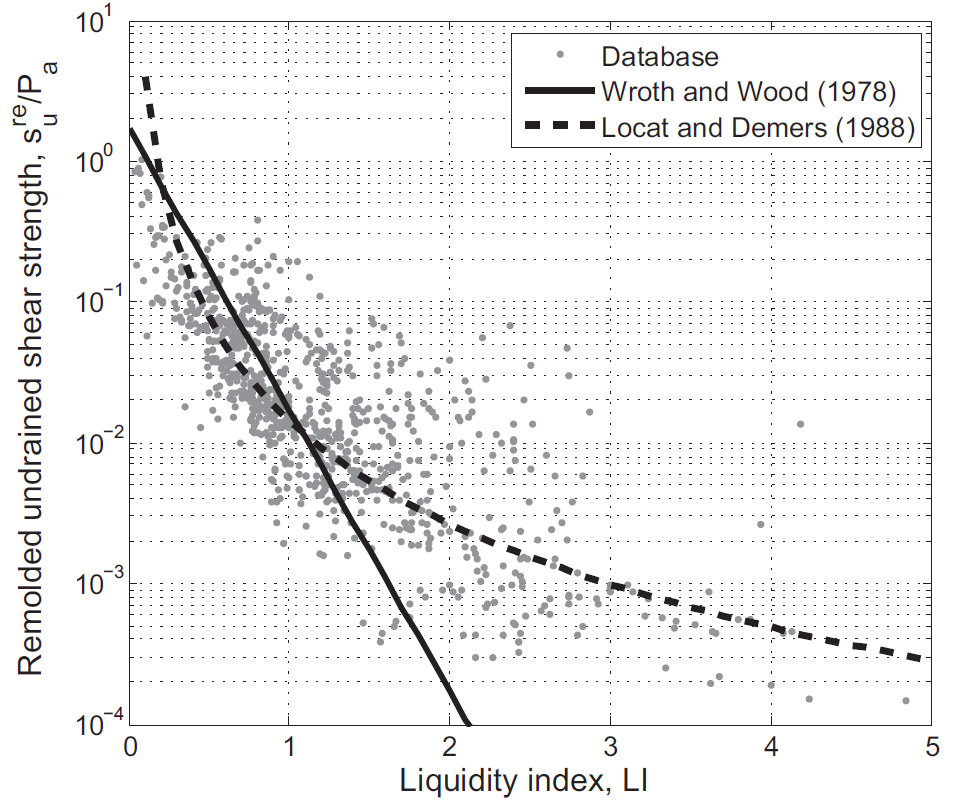
\includegraphics[width=\textwidth]{figures/figure-2.png}
        \caption{$\rm{LI}-(s_u^{re}/P_a)$ models proposed by \citet{Wroth1978137} and \citet{Locat1988799}.}
        \vspace{-5pt}
        \addtocounter{figure}{-1}
        \renewcommand{\figurename}{图}
        \caption{\citet{Wroth1978137}和\citet{Locat1988799}提出的$\rm{LI}-(s_u^{re}/P_a)$模型。}
        \label{figure:2}
        \renewcommand{\figurename}{Figure}
    \end{minipage}
    \begin{minipage}[t]{0.48\textwidth}
        \centering
        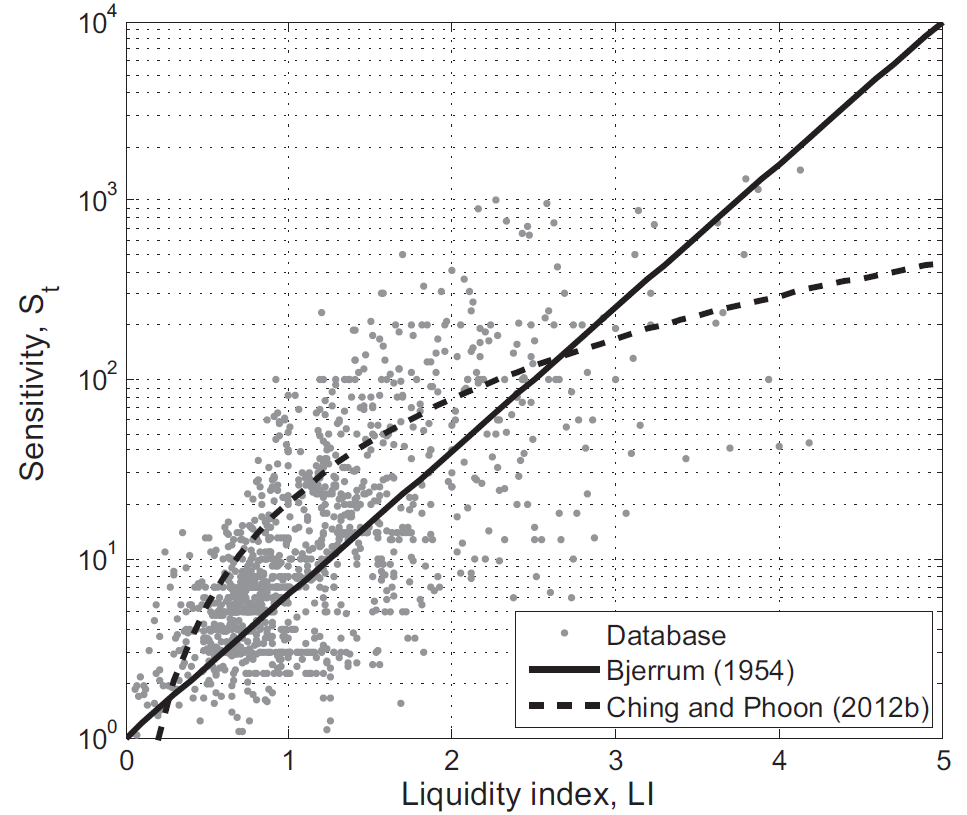
\includegraphics[width=\textwidth]{figures/figure-3.png}
        \caption{$\rm{LI}-S_t$ models proposed by \citet{Bjerrum195449} and \citet{Ching2012522}.}
        \vspace{-5pt}
        \addtocounter{figure}{-1}
        \renewcommand{\figurename}{图}
        \caption{\citet{Bjerrum195449}和\citet{Ching2012522}提出的$\rm{LI}-S_t$模型。}
        \label{figure:3}
        \renewcommand{\figurename}{Figure}
    \end{minipage}
\end{figure*}

\begin{figure*}[!p]
    \centering
    \begin{minipage}[t]{0.48\textwidth}
        \centering
        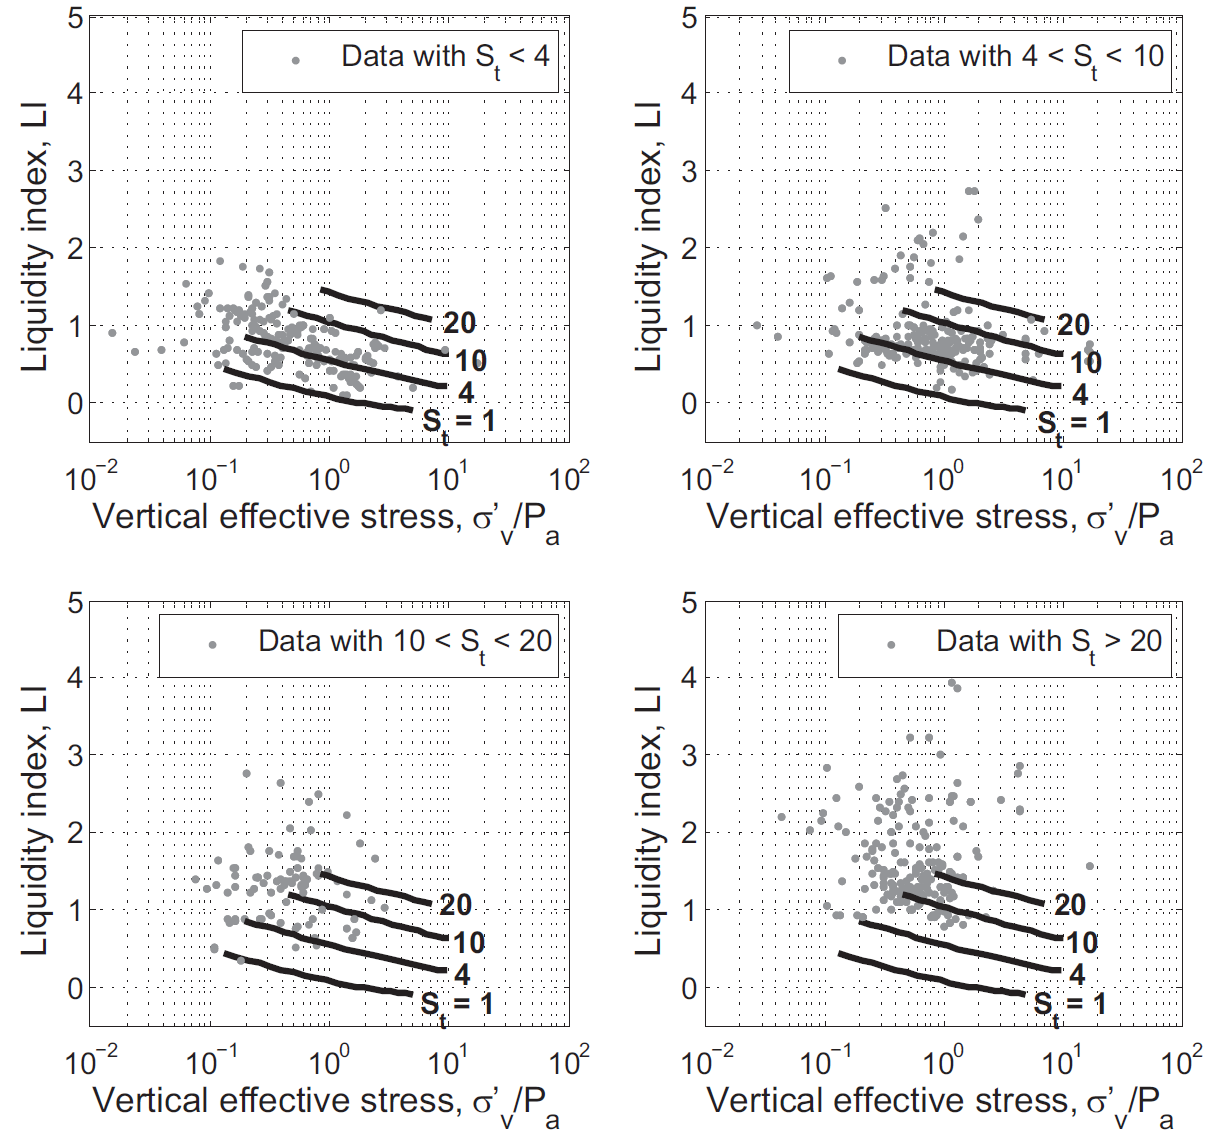
\includegraphics[width=\textwidth]{figures/figure-4.png}
        \caption{$\rm{LI}-(\sigma_v'/P_a)-S_t$ model proposed by \citet{Mitchell1993}.}
        \vspace{-5pt}
        \addtocounter{figure}{-1}
        \renewcommand{\figurename}{图}
        \caption{\citet{Mitchell1993}提出的$\rm{LI}-(\sigma_v'/P_a)-S_t$模型。}
        \label{figure:4}
        \renewcommand{\figurename}{Figure}
    \end{minipage}
    \begin{minipage}[t]{0.48\textwidth}
        \centering
        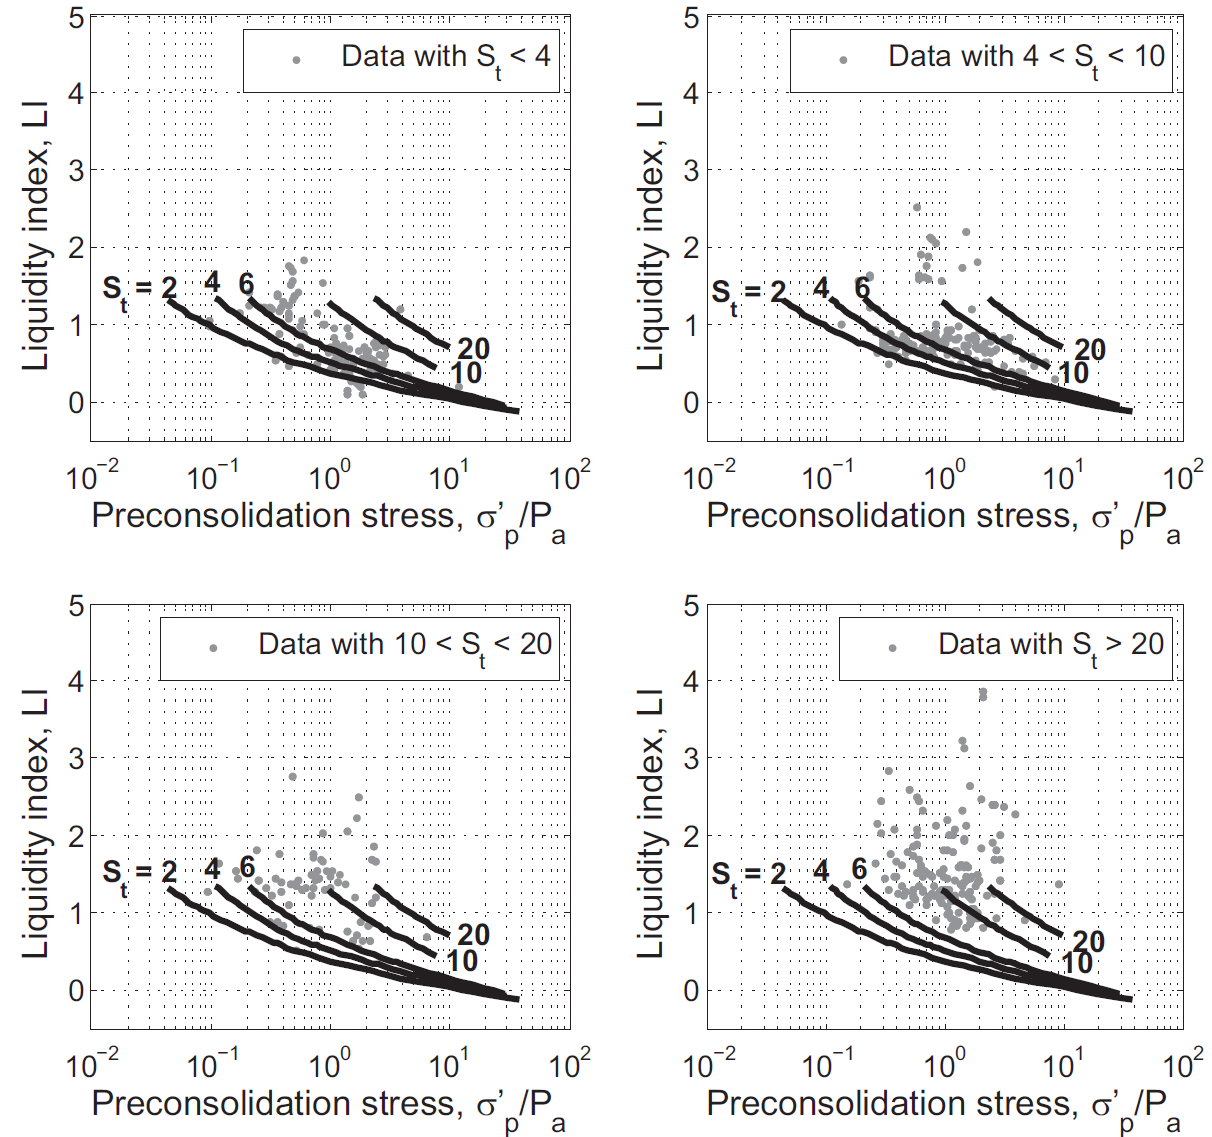
\includegraphics[width=\textwidth]{figures/figure-5.png}
        \caption{$\rm{LI}-(\sigma_p'/P_a)-S_t$ models proposed by \citet{NAVFAC1982}.}
        \vspace{-5pt}
        \addtocounter{figure}{-1}
        \renewcommand{\figurename}{图}
        \caption{\citet{NAVFAC1982}提出的$\rm{LI}-(\sigma_p'/P_a)-S_t$模型。}
        \label{figure:5}
        \renewcommand{\figurename}{Figure}
    \end{minipage}
\end{figure*}

\begin{figure*}[!p]
    \centering
    \begin{minipage}[t]{0.48\textwidth}
        \centering
        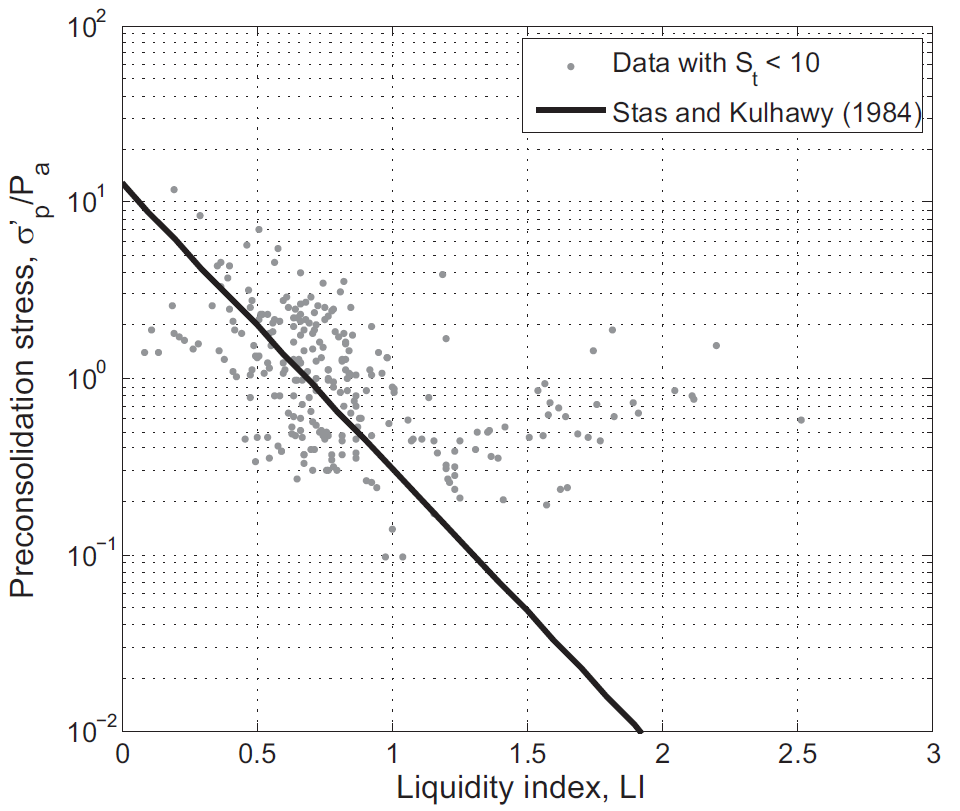
\includegraphics[width=\textwidth]{figures/figure-6.png}
        \caption{$\rm{LI}-(\sigma_p'/P_a)-S_t$ model proposed by \citet{Stas1984}.}
        \vspace{-5pt}
        \addtocounter{figure}{-1}
        \renewcommand{\figurename}{图}
        \caption{\citet{Stas1984}提出的$\rm{LI}-(\sigma_p'/P_a)-S_t$模型。}
        \label{figure:6}
        \renewcommand{\figurename}{Figure}
    \end{minipage}
    \begin{minipage}[t]{0.48\textwidth}
        \centering
        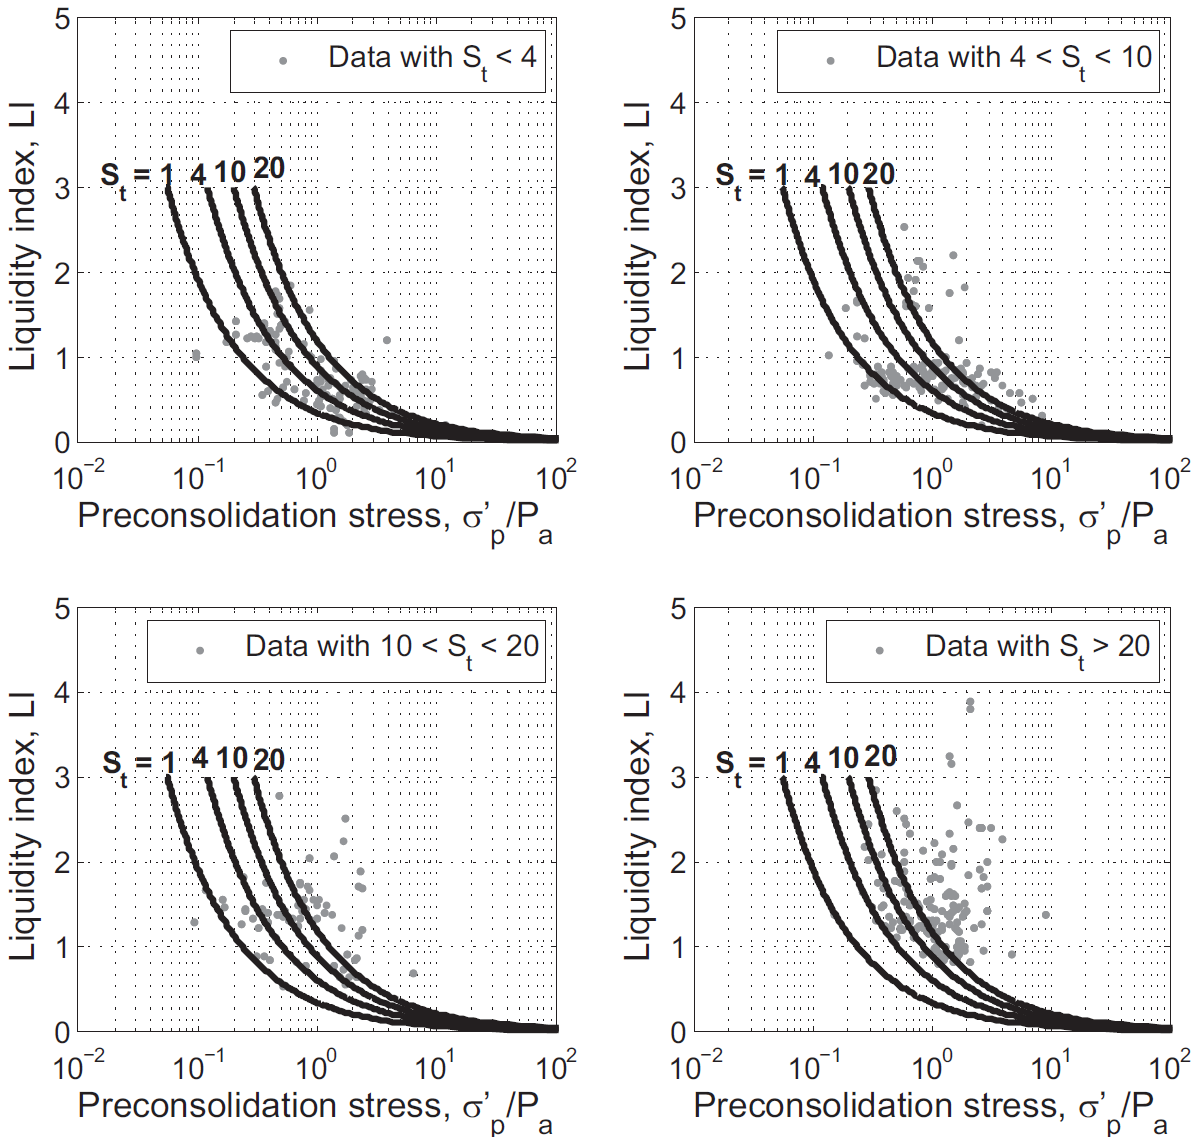
\includegraphics[width=\textwidth]{figures/figure-7.png}
        \caption{$\rm{LI}-(\sigma_p'/P_a)-S_t$ models proposed by \citet{Ching2012522}.}
        \vspace{-5pt}
        \addtocounter{figure}{-1}
        \renewcommand{\figurename}{图}
        \caption{\citet{Ching2012522}提出的$\rm{LI}-(\sigma_p'/P_a)-S_t$模型。}
        \label{figure:7}
        \renewcommand{\figurename}{Figure}
    \end{minipage}
\end{figure*}

\begin{figure*}[!p]
    \centering
    \begin{minipage}[t]{0.48\textwidth}
        \centering
        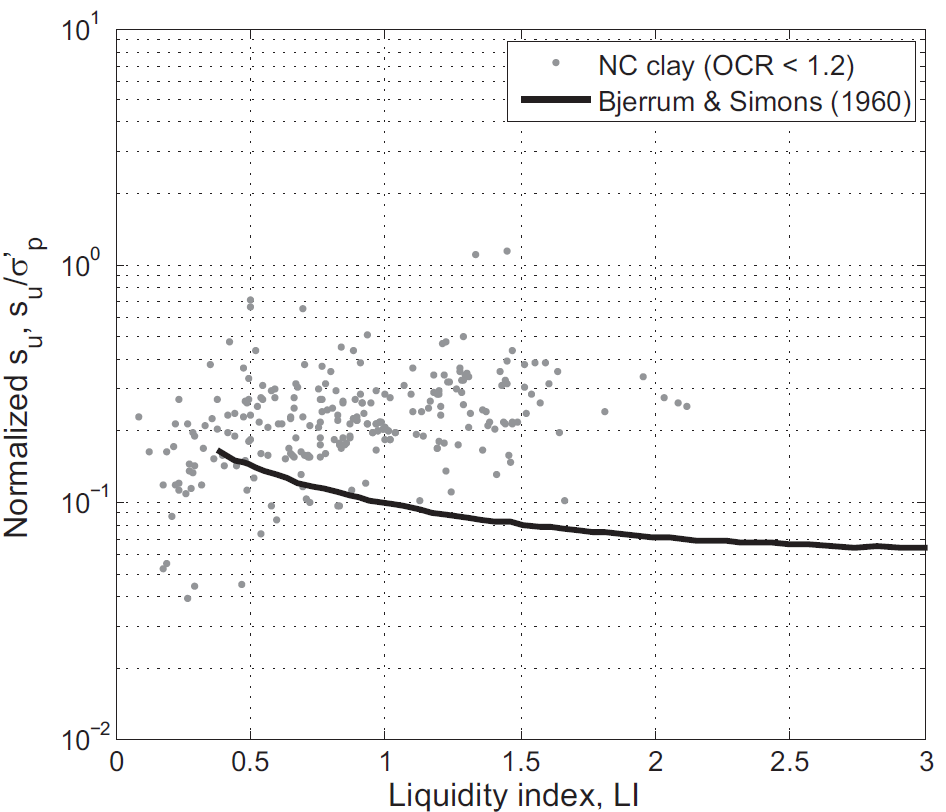
\includegraphics[width=\textwidth]{figures/figure-8.png}
        \caption{$\rm{LI}-(s_u/\sigma_p')$ model proposed by \citet{Bjerrum1960711}.}
        \vspace{-5pt}
        \addtocounter{figure}{-1}
        \renewcommand{\figurename}{图}
        \caption{\citet{Bjerrum1960711}提出的$\rm{LI}-(s_u/\sigma_p')$模型。}
        \label{figure:8}
        \renewcommand{\figurename}{Figure}
    \end{minipage}
    \begin{minipage}[t]{0.48\textwidth}
        \centering
        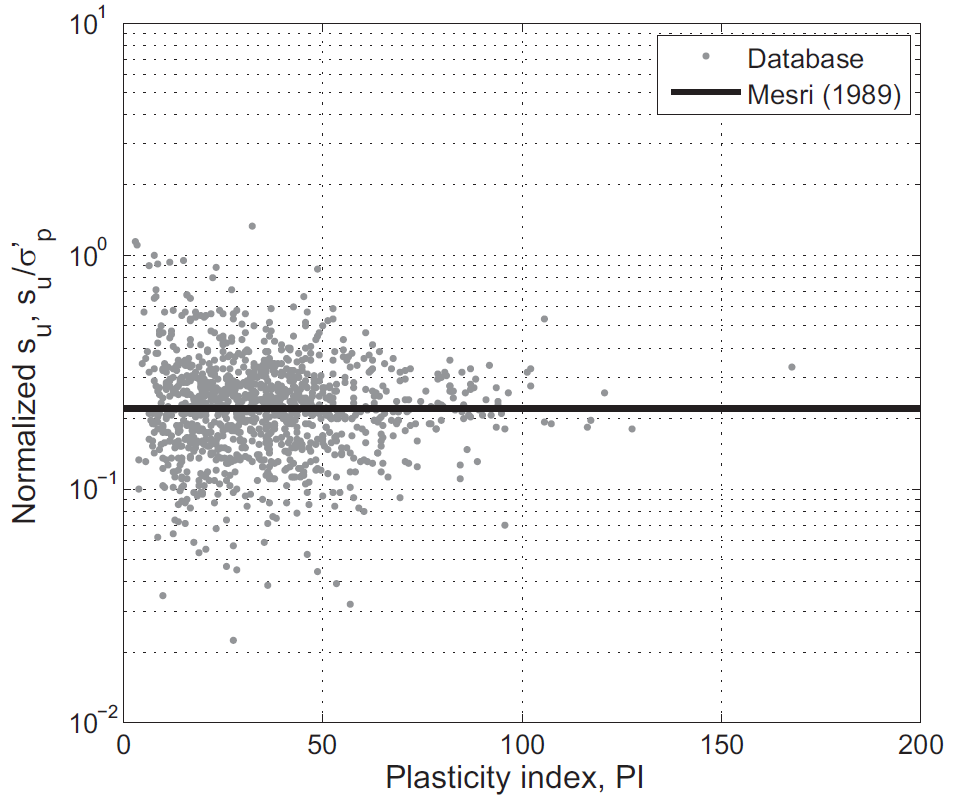
\includegraphics[width=\textwidth]{figures/figure-9.png}
        \caption{$\rm{LI}-(s_u/\sigma_p')$ models proposed by \citet{Mesri1975409, Mesri1989162}.}
        \vspace{-5pt}
        \addtocounter{figure}{-1}
        \renewcommand{\figurename}{图}
        \caption{\citet{Mesri1975409, Mesri1989162}提出的$\rm{LI}-(s_u/\sigma_p')$模型。}
        \label{figure:9}
        \renewcommand{\figurename}{Figure}
    \end{minipage}
\end{figure*}

\begin{figure*}[!p]
    \centering
    \begin{minipage}[t]{0.48\textwidth}
        \centering
        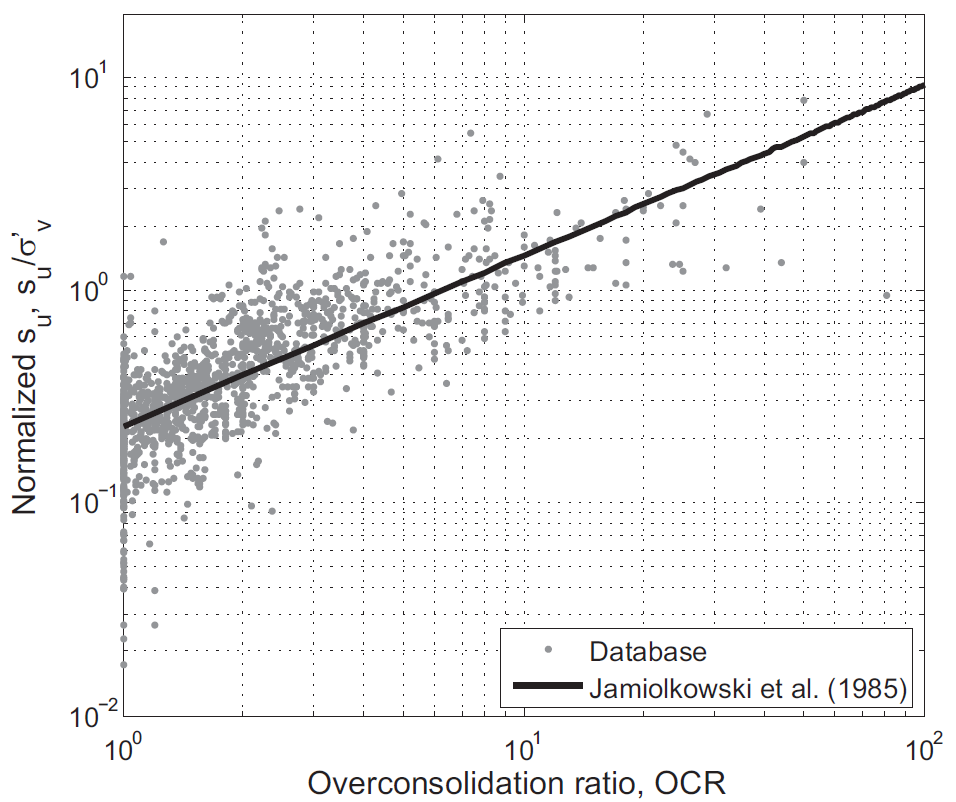
\includegraphics[width=\textwidth]{figures/figure-10.png}
        \caption{$\rm{OCR}-(s_u/\sigma_p')$ model proposed by \citet{Jamiolkowski198557}.}
        \vspace{-5pt}
        \addtocounter{figure}{-1}
        \renewcommand{\figurename}{图}
        \caption{\citet{Jamiolkowski198557}提出的$\rm{OCR}-(s_u/\sigma_p')$模型。}
        \label{figure:10}
        \renewcommand{\figurename}{Figure}
    \end{minipage}
    \begin{minipage}[t]{0.48\textwidth}
        \centering
        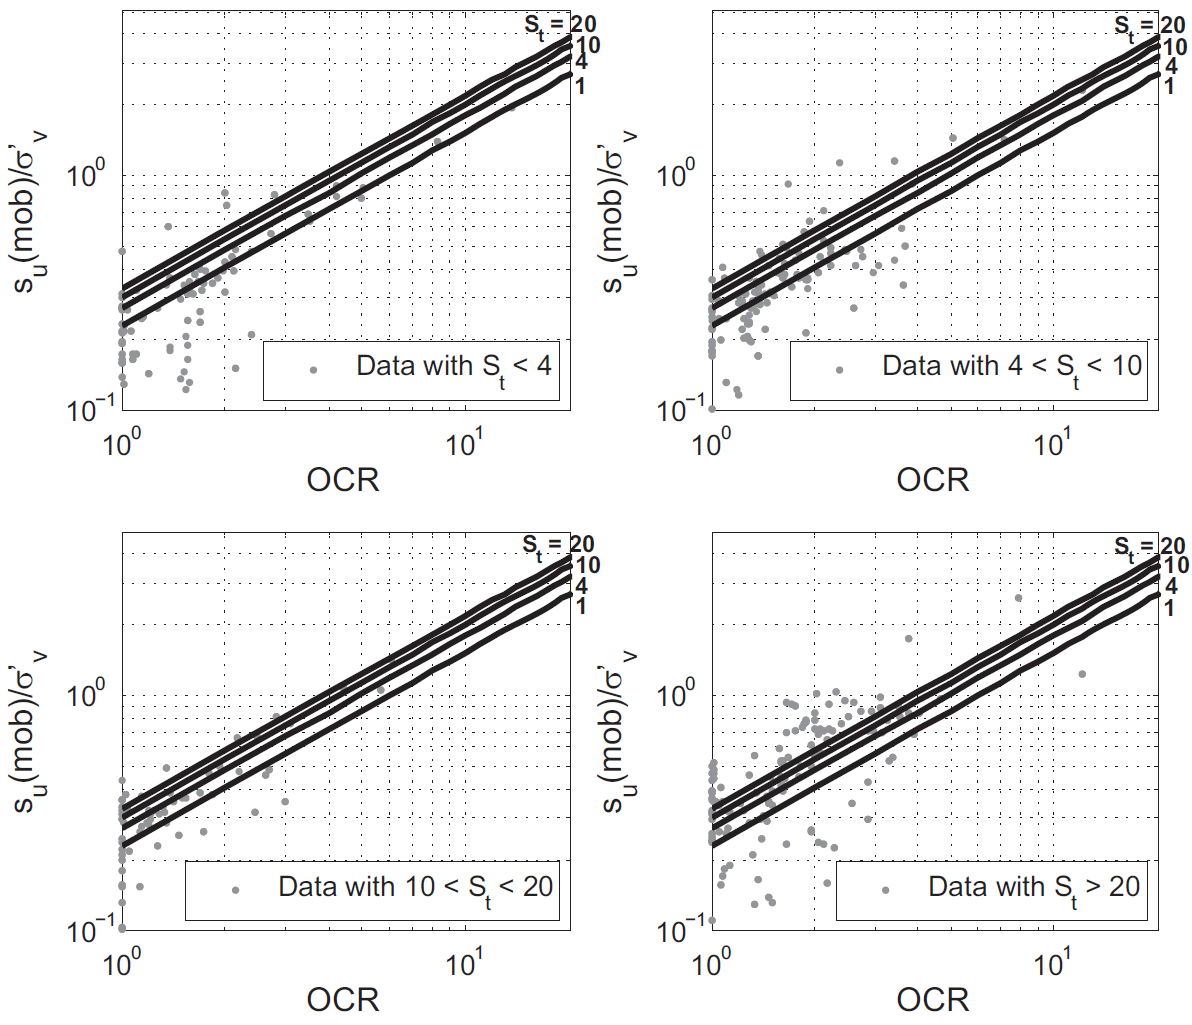
\includegraphics[width=\textwidth]{figures/figure-11.png}
        \caption{$\rm{OCR}-(s_u/\sigma_p')-S_t$ models proposed by \citet{Ching2012522}.}
        \vspace{-5pt}
        \addtocounter{figure}{-1}
        \renewcommand{\figurename}{图}
        \caption{\citet{Ching2012522}提出的$\rm{OCR}-(s_u/\sigma_p')-S_t$模型。}
        \label{figure:11}
        \renewcommand{\figurename}{Figure}
    \end{minipage}
\end{figure*}

\begin{figure*}[!p]
    \centering
    \begin{minipage}[t]{0.48\textwidth}
        \centering
        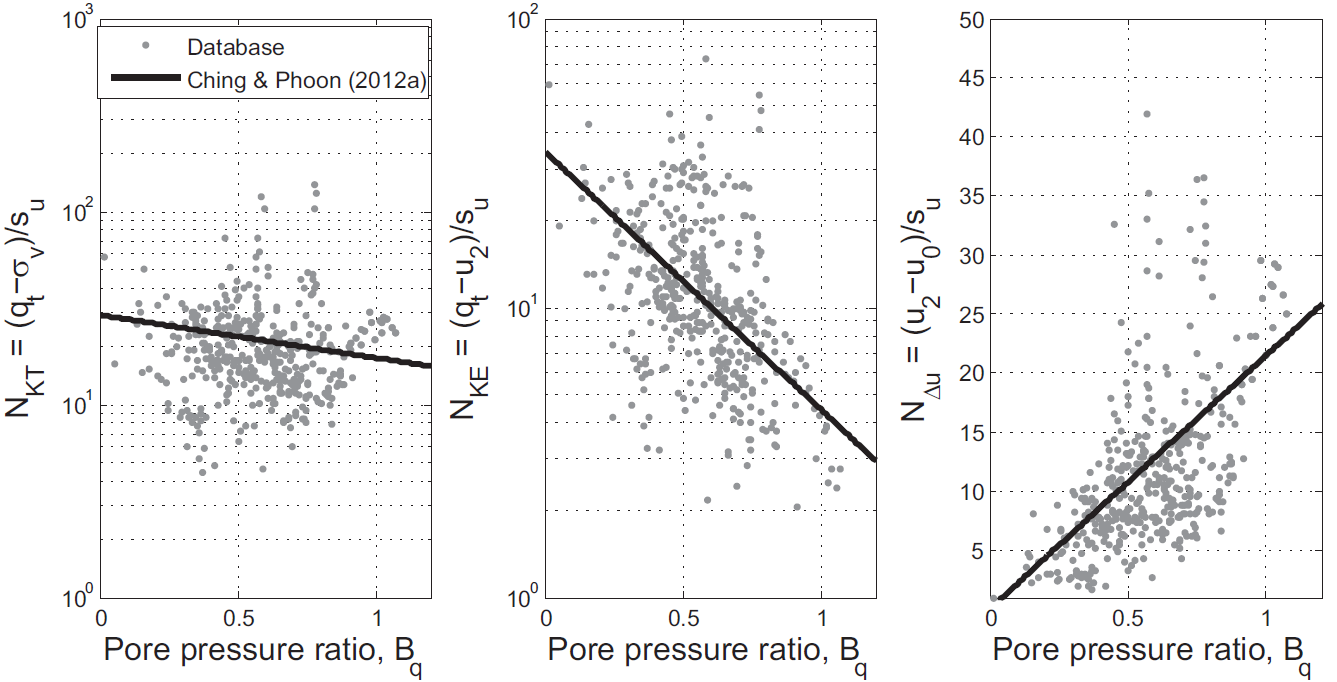
\includegraphics[width=\textwidth]{figures/figure-12.png}
        \caption{$\rm{CPTU}-s_u/\sigma_v'$ model proposed by \citet{Ching2012522}.}
        \vspace{-5pt}
        \addtocounter{figure}{-1}
        \renewcommand{\figurename}{图}
        \caption{\citet{Ching2012522}提出的$\rm{CPTU}-s_u/\sigma_v'$模型。}
        \label{figure:12}
        \renewcommand{\figurename}{Figure}
    \end{minipage}
    \begin{minipage}[t]{0.48\textwidth}
        \centering
        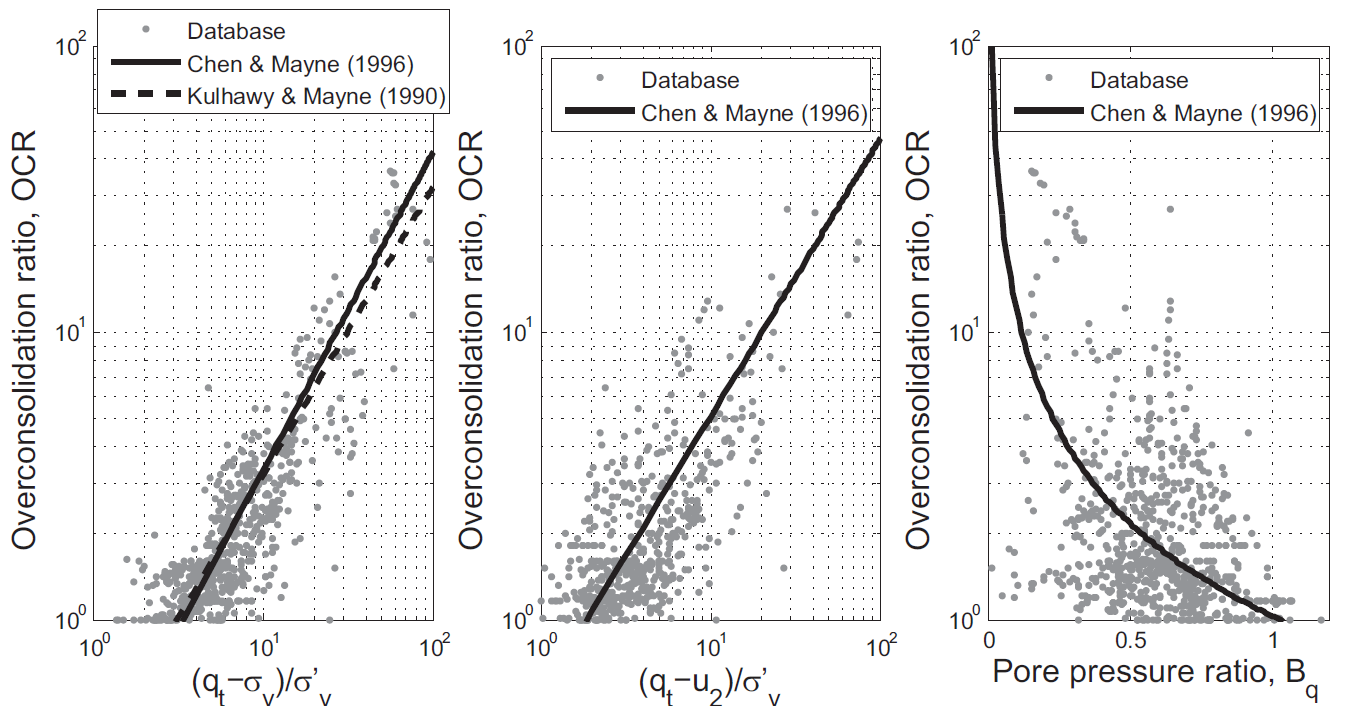
\includegraphics[width=\textwidth]{figures/figure-13.png}
        \caption{CPTU-OCR model proposed by \citet{Chen1996488, Kulhawy1990}.}
        \vspace{-5pt}
        \addtocounter{figure}{-1}
        \renewcommand{\figurename}{图}
        \caption{\citet{Chen1996488, Kulhawy1990}提出的CPTU-OCR模型。}
        \label{figure:13}
        \renewcommand{\figurename}{Figure}
    \end{minipage}
\end{figure*}

\begin{figure*}[!p]
    \centering
    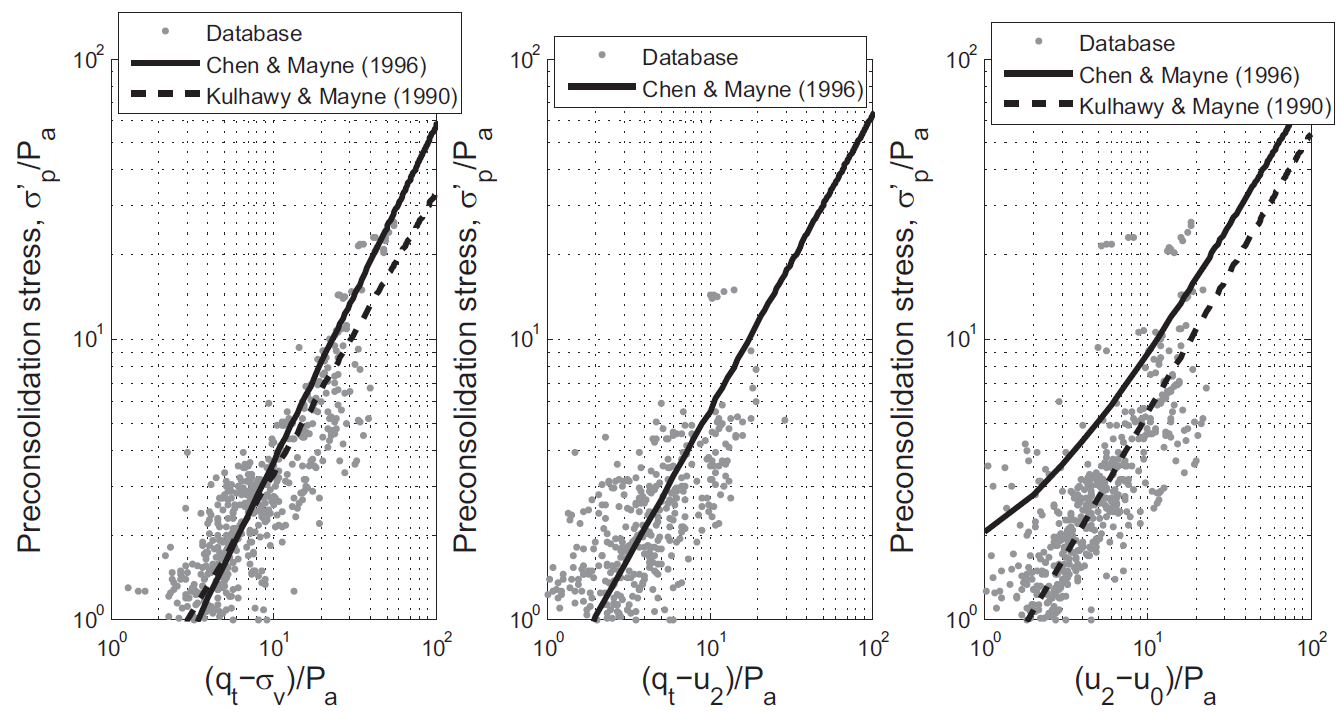
\includegraphics[width=0.5\textwidth]{figures/figure-14.png}
    \caption{$\rm{CPTU}-\sigma_p'/P_a$ model proposed by \citet{Chen1996488, Kulhawy1990}.}
    \vspace{-5pt}
    \addtocounter{figure}{-1}
    \renewcommand{\figurename}{图}
    \caption{\citet{Chen1996488, Kulhawy1990}提出的$\rm{CPTU}-\sigma_p'/P_a$模型。}
    \label{figure:14}
    \renewcommand{\figurename}{Figure}
\end{figure*}

    \switchcolumn*
        
    The comparison results between the transformation models and the database are shown in \autoref{figure:2}–\autoref{figure:14}. For the models with a secondary input parameter St, data points in our database are divided into four groups according to their St values, and four subplots are presented to compare with the transformation models. The four groups are obtained based on St < 4, 4 < St < 10, 10 < St < 20, and St > 20. \autoref{figure:2}~–~\autoref{figure:14} show that the global data follow similar trends to most transformation models reported in the literature. The exceptions are the following six models:
    \begin{enumerate}
        \item The $\rm{LI}-(s_u^{re}/P_a)$ model proposed by \citet{Wroth1978137}. This model was developed based on the modified Cam Clay model. It provides a reasonable average fit to the data for LI < 1 as shown in \autoref{figure:2}. However, it deviates significantly from the data points in our global database for LI > 1.5.
        
        \item The $\rm{LI}-(\sigma_v'/P_a)-S_t$ model proposed by \citet{Mitchell1993}. Despite the wide scatter as shown in \autoref{table:4}, there is general agreement between this model and the global data for data points with 4 < St < 20. However, for data with small St values (St < 4) or with large St values (St > 20), the agreement is poor. It is possible that this model was developed with most data points falling between 4 < St < 20. In other words, the empirical support for small and large St values may be weak.
        
        \item The $\rm{LI}-(\sigma_p'/P_a)-S_t$ model proposed by \citet{NAVFAC1982}. The observations here are similar to those for the Mitchell’s model: there is a reasonably good agreement between the model and the global data for data points with 4 < St < 20 (see \autoref{figure:5}). The agreement is poor outside this range of St. One may venture to guess that the empirical support for small and large St values is also weak for this model.
        
        \item The $\rm{LI}-(\sigma_p'/P_a)-S_t$ model proposed by \citet{Ching2012522}. The agreement between this model and the global data are reasonable for data points with large St values (St > 20) as shown in \autoref{figure:7}. However, this model does not fit data with small St values (St < 4). This is because the database CLAY/5/345 used to develop this $\rm{LI}-(\sigma_p'/P_a)-S_t$ model contains only structured clays.
        
        \item $\rm{LI}-(s_u/\sigma_p')$ model proposed by \citet{Bjerrum1960711}. In \autoref{figure:8}, only data points with OCR < 1.2 (nearly NC clays) in the global database are plotted. Nonetheless, the discrepancy between the model and the data is clear. Note that this model was developed based on Norwegian NC clays only. It is most likely that this site-specific model fits to the Norwegian data, but not to the global data from diverse geographic origins.
        
        \item One of the $\rm{CPTU}-(\sigma_p'/P_a)$ models proposed by \citet{Chen1996488} (the third model that relates $\sigma_p'$ to $(u_2-u_0)/P_a$ in \autoref{table:5}). The discrepancy between this model and our global data is apparent. However, the first two models developed by \citet{Chen1996488} (the two models that relate $\sigma_p'/P_a$ to $(q_t-\sigma_v)/P_a$ and $(q_t-u_2)/P_a$) provide reasonable fits to our global data. We are unable to explain this anomaly.
    \end{enumerate}

    \switchcolumn
        
    转换模型与数据库的比较结果如\cnfigureref{figure:2}-\cnfigureref{figure:14}所示。 对于具有辅助输入参数St的模型,我们数据库中的数据点根据其St值分为四组,并提出了四个子图与转换模型进行比较。 根据St < 4,4 <St <10,10 <St <20和St > 20获得这四个组。\cnfigureref{figure:2}–\cnfigureref{figure:14}显示,全球数据遵循与文献中报道的大多数转换模型相似的趋势。 以下六个模型除外:
    \begin{enumerate}
        \item \citet{Wroth1978137}提出的$\rm{LI}-(s_u^{re}/P_a)$模型。该模型是基于修改后的Cam Clay模型开发的。如\cnfigureref{figure:2}所示,它为LI < 1的数据提供了合理的平均拟合。但是,对于我们的LI > 1.5,它与我们的全局数据库中的数据点有很大的出入。
        
        \item \citet{Mitchell1993}提出的$\rm{LI}-(\sigma_v'/P_a)-S_t$模型。尽管如\cnfigureref{table:4}所示分散范围很广,但是对于4 <St <20的数据点,该模型与全局数据之间存在普遍共识。但是,对于St值小的(St < 4)或St值大的数据(St > 20),匹配性很差。该模型可能是在大多数数据点落在4 < St < 20之间的情况下开发的。换句话说,对小和大的St值的经验支持可能很弱。
        
        \item \citet{NAVFAC1982}提出的$\rm{LI}-(\sigma_p'/P_a)-S_t$模型。这里的观察结果与Mitchell模型的观察结果相似:对于4 < St <20的数据点,模型与全局数据之间存在相当好的一致性(见\cnfigureref{figure:5})。在St的这一范围之外,该匹配的效果很差。有人可能会猜测,对于该模型,对于小和大的St值的经验支持也很弱。
        
        \item \citet{Ching2012522}提出的$\rm{LI}-(\sigma_p'/P_a)-S_t$模型。如\cnfigureref{figure:7}所示,此模型与全局数据之间的一致性对于具有较大St值(St > 20)的数据点是合理的。但是,此模型不适用于具有较小St值(St < 4)的数据。这是因为用于开发此$\rm{LI}-(\sigma_p'/P_a)-S_t$模型的数据库CLAY/5/345仅包含结构化粘土。
        
        \item \citet{Bjerrum1960711}提出的$\rm{LI}-(s_u/\sigma_p')$模型。在\cnfigureref{figure:8}中,仅绘制了全局数据库中OCR < 1.2(接近NC黏土)的数据点。尽管如此,模型和数据之间的差异仍然很明显。请注意,此模型仅基于挪威NC黏土开发。此特定于站点的模型很可能适合挪威的数据,但不适合来自不同地理来源的全球数据。
        
        \item \citet{Chen1996488}提出的$\rm{CPTU}-(\sigma_p'/P_a)$模型之一(\cntableref{table:5}中$\sigma_p'$与$(u_2-u_0)/P_a$相关的第三种模型)。该模型与我们的全局数据之间的差异显而易见。然而,由\citet{Chen1996488}开发的前两个模型($\sigma_p'/P_a$与$(q_t-\sigma_v)/P_a$相关的模型和$(q_t-u_2)/P_a$模型)合理地拟合了我们的全球数据。我们无法解释这种异常。
    \end{enumerate}

\end{paracol}